\section{Try Resource}

Com o advento do Java 7 foi introduzido o \textit{Try with Resource} com isso promoveu uma maior autonomia e flexibilidade ao programador. Foi encontrado no total 284321 \textit{trys} nos quais já estão com a essa \textit{feature} são somente 5186. Como mostra na imagem abaixo mostra que dos projetos que foram analisados somente esses 4 projetos fazem algum uso dessa estrutura mas fica predominantemente no Jboss que é um servidor de aplicação o que mostra que a comunidade não adotou essa \textit{feature} com peso.\\ 


\begin{figure}[h]
	\center
	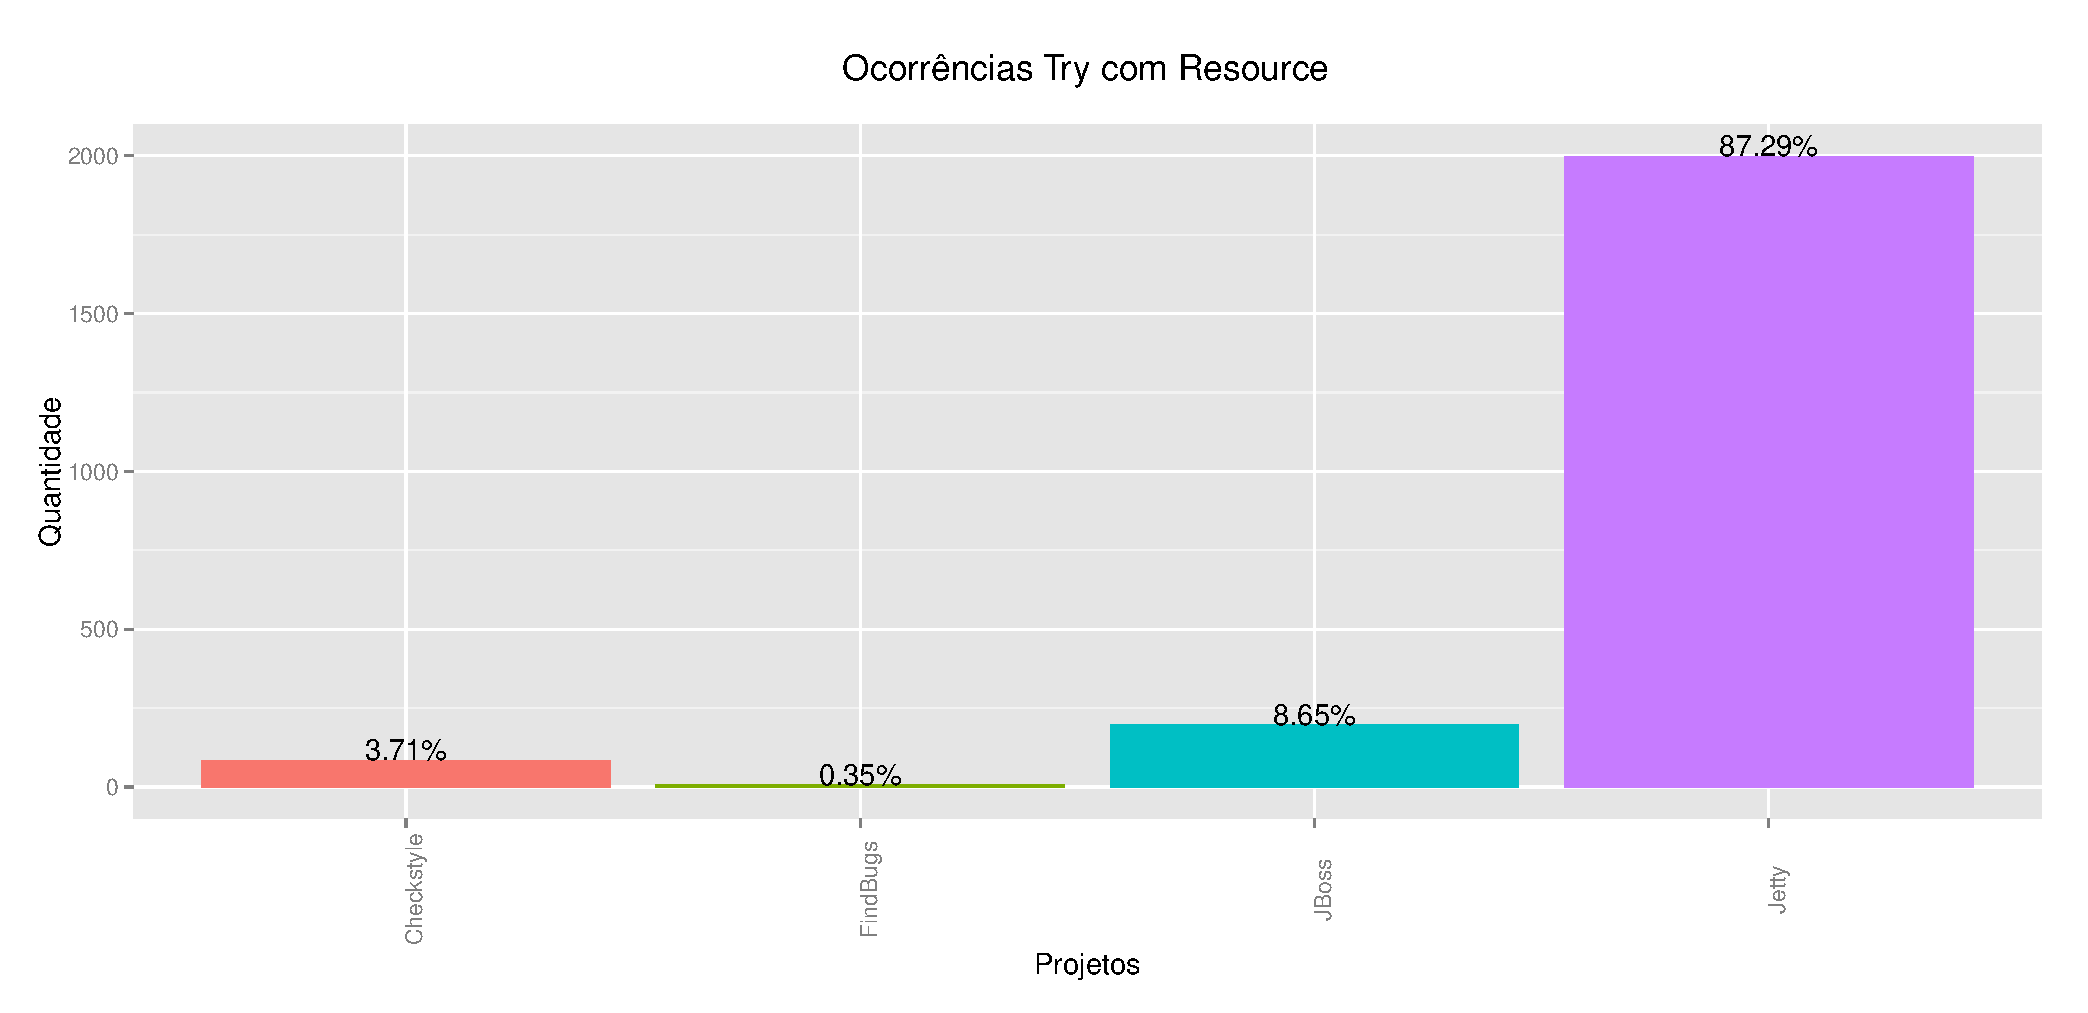
\includegraphics[scale=0.5]{Imagens/ocorrenciasTryResource}
	\label{fig:Try with Resource}
	\caption{Oportunidades de \textit{Try with Resource} nos projetos.}
\end{figure}
\clearpage